\documentclass[conference,letterpaper]{IEEEtran}

\usepackage[utf8]{inputenc}
\usepackage{cite}
\usepackage[pdftex]{graphicx}
\usepackage{url}
\usepackage{csquotes}
\usepackage{dblfloatfix}
\usepackage{hyperref}
\usepackage{soul}

\begin{document}
\title{Distributing Distributed Revision Control Systems}

\author{\IEEEauthorblockN{Philipp Hagemeister}
\IEEEauthorblockA{Heinrich-Heine-Universität Düsseldorf\\
Email: hagemeister@cs.uni-duesseldorf.de}
\and
\IEEEauthorblockN{Martin Mauve}
\IEEEauthorblockA{Heinrich-Heine-Universität Düsseldorf\\
Email: mauve@cs.uni-duesseldorf.de}
}
\maketitle


\begin{abstract}
\boldmath Current revision control systems are commonly used in a distributed fashion but rely on centralized stores and low-latency communication. In this work we evaluate how they would fare in fully distributed high latency networks such as delay tolerant networks (DTNs). We show that current revision control systems impose significant costs under these conditions even in moderately-sized networks. By simplifying/improving the merging process, these costs can be reduced.
We also show that speeding up \textit{or slowing down} communication can reduce the costs significantly.
\end{abstract}

\IEEEpeerreviewmaketitle

\section{Introduction}

Joint work on text documents is a cornerstone of political activities in a democracy. For example, drafting the program of a party, preparing proposals for laws and regulations, gathering feedback on what collective actions should be taken requires read and write access to shared text documents. Revision control systems are a fundamental tool to support this kind of cooperation.

However, as we have seen during the Arab spring, Egypt and Libya effectively shut down their Internet access\cite{outage}. China and Iran, among others, also employ sophisticated Internet censorship, which could prevent such cooperation.

While Internet access is typically centralized and can therefore be censored easily, distributed systems where users communicate peer-to-peer are exceptionally hard to censor. Therefore, we want to enable revision control systems to work in the face of censorship by using them in a distributed fashion.

We envision a scenario where numerous groups of users meet up and create a common document using local WiFi and then transmit the changes via \textit{sneakernet}\footnote{e.g. USB thumb drives} or local networks. Some users may simultaneously be able to communicate with a central server or Internet-based peer-to-peer network, but there is no single master copy. Instead, new changes get integrated into the local state when they become available via any communication channel.

Current revision control systems such as \textit{git} do include support for a distributed way of working and are hence often called distributed, but in practice use one or a very small number of centralized stores to synchronize the users' work. If such a centralized store is not available -- for example because of censorship -- this workflow breaks down. The flow of data in a distributed system is completely different, and neccesitates the analysis of potential pitfalls which we want to provide in this paper.

Current peer-to-peer revision control systems such as PlatinVC\cite{mukherjee2005fully} or TierStore\cite{demmer2008tierstore} already automate the synchronization process by selecting one node to synchronize the most current version across the network. While this approach is distributed, it only works in low-latency networks. However, the networks we are envisioning have very high latencies because users need to physically move in order to be able to communicate. Parts of the networks may be low-latency (for example, a group of democratic leaders at a retreat), but in general, our network is a Delay~Tolerant~Network~(DTN).

We want to know whether such a revision control system can work when there is no central synchronization point, and under what conditions it works best.

In the remainder of the paper we investigate how the mechanisms used in current revision control systems would work in a setting where there is no central synchronization point and the communication channel has a very high latency. To this end we use network simulation as this allows us to experiment with a large number of different settings and get a good first understanding of the key issues involved.

\section{Simulation Setup}

A graph-based revision control system can be modeled as a directed acyclic graph (DAG) of commits by a pool of $n$ users. There is an empty root commit common to the project. For every user, there is always one newest commit in the DAG. Every edit brings about a new commit based upon the newest existing locally visible DAG. When a node sends its current DAG to another node, the receiving node will make sure to merge it to get to one newest node. Fig. \ref{fig:grcs} presents a simple example of the DAG in a revision control system.

Merging typically requires user interaction (arguably the costliest resource in such a system), because the user may have to find a compromise between two (the local and the just-received) differing versions, each version being the top of a subgraph of the DAG of all versions. Merging is necessary not only because it allows the user to see the newest state of the system, but also because it is fundamental in unifying differing points. For instance, Alice may divide a run-on sentence with a semicolon, whereas Bob uses a period. Upon merging, someone (whoever is merging) must decide which one to pick.

\begin{figure}
  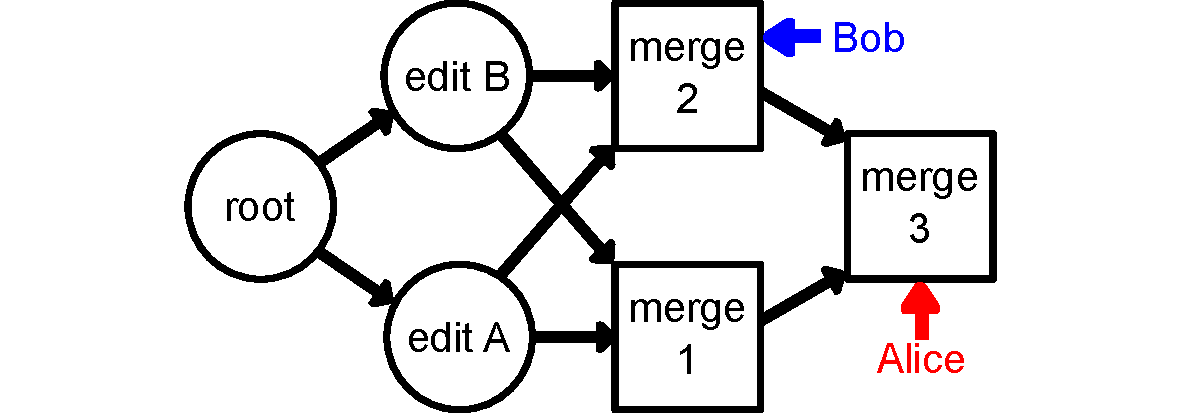
\includegraphics[width=\linewidth]{img_pdf/grcs.pdf}
  \caption{Example of a very simple revision history. Alice and Bob have authored edit A and B, respectively. They sent their edits to each other concurrently, and each created a merge. Alice then got Bob's merge 1, and merged it with her merge 2. The newest node of Bob is merge 2; the newest node of Alice is merge 3. If Bob now learns of merge 3, he will simply update his \textit{newest node} pointer to merge 3.}
  \label{fig:grcs}
\end{figure}

To characterize the merging, we look at the two current commits (each forming the top of a sub-DAG) to merge and distinguish two basic cases: If one of the top commits is an ancestor of the other -- including both top commits being identical -- then merging is simple, as it only consists of settings the top of the local DAG to the newer of the two commits.

If not, then we can model a wide variety of different merging approaches. With an \textit{ideal} merging function, all merges of a set of edits would result in the same final result, no matter the order and paths that all individual commits got merged in (this is unrealistic, but a good upper boundary on efficiency). At the opposite end of the scale, the \textit{default} approach -- named so because it is the one actually used in practice by graph-based revision control systems at the moment -- simply merges every time it encounters two commits created contemporaneously, providing an upper boundary for the worst possible algorithm. However, note that this accurately models the current state of revision control software.

In both approaches, the final cost is the number of merges in the system, doing double duty both as an indicator of computation/user time as well as network storage requirements.

We assume that nodes meet randomly with exponentially distributed interarrival times per node, which has been shown to be a good modeling for mobile ad-hoc/opportunistic networks\cite{groenevelt}. Due to the speed of WiFi/USB in relation to our textual data, we assume that all transfers are complete.

For the edits, we evaluated both uniform and exponential distributions. Since our timescale is arbitrary (one unit could be hours just as well as minutes), we fixed the expected value of edits to one per time unit.

We divide the simulation into two phases: In the \textit{active} phase, nodes move around and edit the repository, modeling a repository where new content is constantly being added. The active phase is followed by the \textit{cooldown} phase, in which nodes cease to edit new content, but still move around and merge. By examining the behavior in the absence of content generation in the cooldown phase, we can exclude systems that fail on their own, without any input. In addition, the cooldown phase provides a lower boundary for the number of merges a new user would have to perform to reach the most updated state.

\section{Simulation Results}

In general, we ran every simulation 1000 times, taking care not to reuse any numbers out of the random number generator. The simulation code -- including the random seed data -- is published under an open-source license on \url{https://github.com/hhucn/rcssim}.

First of all, we look at how the default algorithm performs in the cooldown phase, i.e. in the absence of actual edits. With a small number of nodes and every node receiving data about once per time unit on average, we can evaluate when we see the final merge in a simulation. We terminate all simulations at time 500 no matter whether convergence has been achieved at that time or not. As shown in fig. \ref{fig:dumb_sunset}, there is a rapid change between 10 and 14 nodes - when more nodes communicate, there is a good chance that despite the lack of new content, merging continues indefinitely. This is in stark contrast to the ideal system shown in the last two columns of fig. \ref{fig:dumb_sunset}, which stops generating new merge commits very quickly after the drying up of new edits. The latter is to be expected, since the number of merges in the cooldown period with an ideal merging system is bounded by the number of commits that nodes have \textit{not} received so far; once a node is aware of all edits, they will not merge in any new commits.

\begin{figure}
  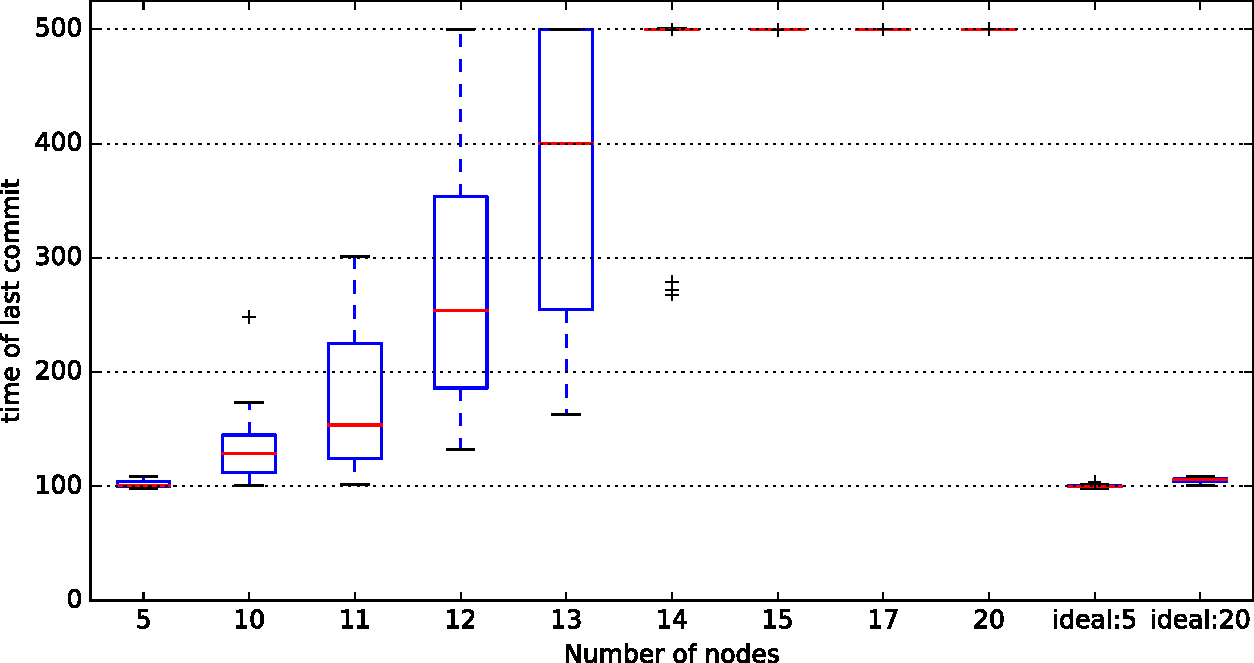
\includegraphics[width=\linewidth]{img_pdf/dumb_sunset_n_scale_last.pdf}
  \caption{Time of last commit with default and ideal merging algorithm}
  \label{fig:dumb_sunset}
\end{figure}

Of course, it is not realistic to assume that actual users will be stuck in an infinite loop and continuously generate new merges (although this may form an accurate description of edit wars). On the other hand, it is also unrealistic that users cease to merge at the instant they see that the edits contained in both sides are identical, even if the final merge result is different. A far more realistic assumption is that users' willingness to merge is dependent on the number of times they have seen the same edits, and thereby the same content. We assume that this willingness decreases exponentially with the number of merges that ultimately pertain to the same edits. We evaluate two scenarios:
Either users ignore new changes (fig. \ref{fig:bored}), or they throw away their own merge(s) and go on with the remote merge (fig. \ref{fig:bored_accept}) in order to achieve unity. Surprisingly, there are no significant differences between both. Most likely, this is because the user's merges already ``escaped" to other users; while competing merges can sometimes be extinguished when they are used, many times all competing merges are still present somewhere in the system.

\begin{figure}
  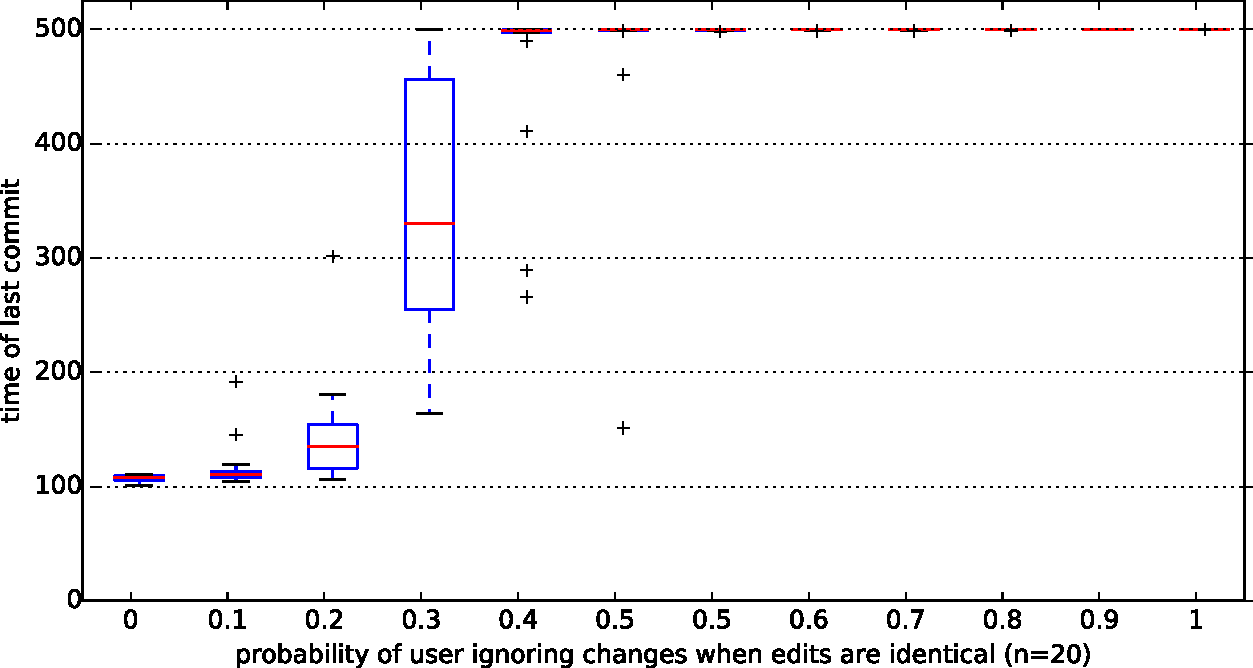
\includegraphics[width=\linewidth]{img_pdf/bored_n=20.pdf}
  \caption{Effect of users ignoring new changes if edits in both commits are identical (0: all commits are ignored, 1: merging every time)}
  \label{fig:bored}
\end{figure}

\begin{figure}
  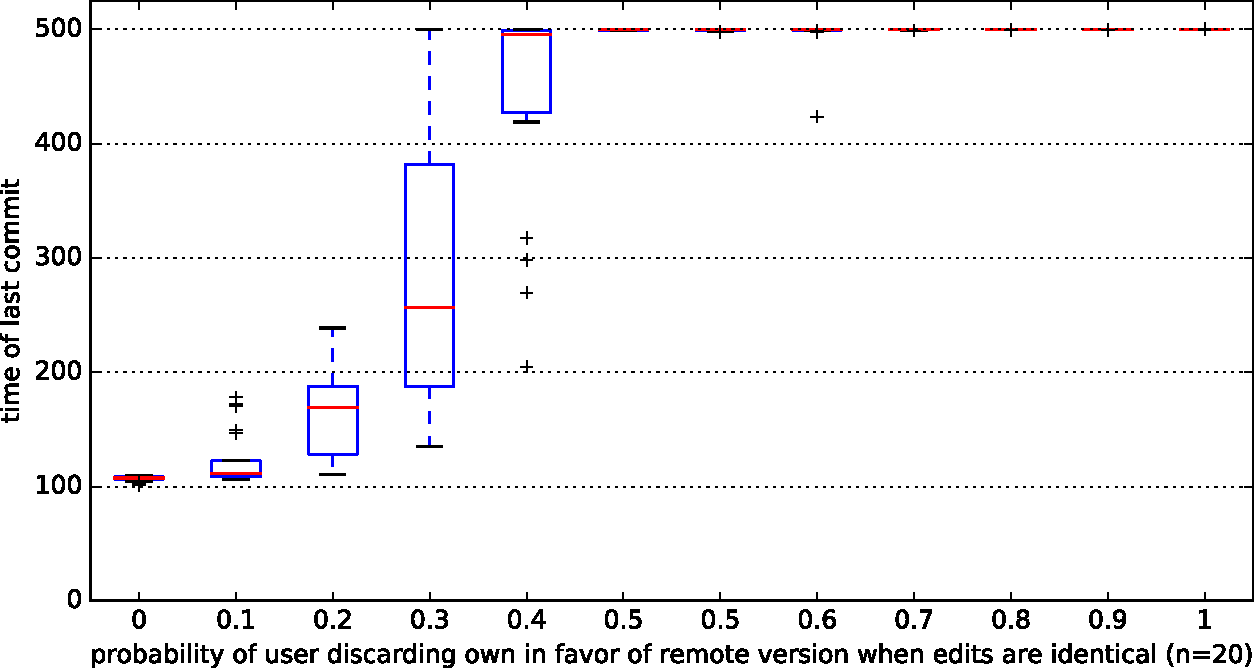
\includegraphics[width=\linewidth]{img_pdf/bored_accept_n=20.pdf}
  \caption{Effect of users simply accepting the remote version when edits in both commits are identical (0: all commits are ignored, 1: merging every time)}
  \label{fig:bored_accept}
\end{figure}

In the rest of the paper, we evaluate how varying rates and forms of editing and network sizes influence the total number of merges. To exclude the inherent accumulation of merges with the default algorithm even in the absence of new edits, we assume an ideal merging function.

By varying the network size as well as rate of meetings and edits, we can discover how revision control systems fare under varying circumstances. In the following set of simulations, we assumed 1 edit per time unit and varied how often node would meet per time unit. The users only merge if the content of the two commits to merge is different, which corresponds to an ideal merging function.

When nodes meet very rarely, the total number of merges is constrained by the meetings; almost every meeting results in a merge. In this scenario, it is also possible that new edits of a node directly follow the previous edits of the same node. On the opposite end, with a high frequency of encounters, there is a good chance that new edits are propagated to the network - just like in an centralized system, all nodes encounter all the edits in the same order. For instance, in the simulation shown in fig. \ref{fig:freq_n10}, we generate 1 edit per time unit somewhere in the whole network. We can plainly see that 1 meeting per time unit causes the maximum number of merges.

\begin{figure}
  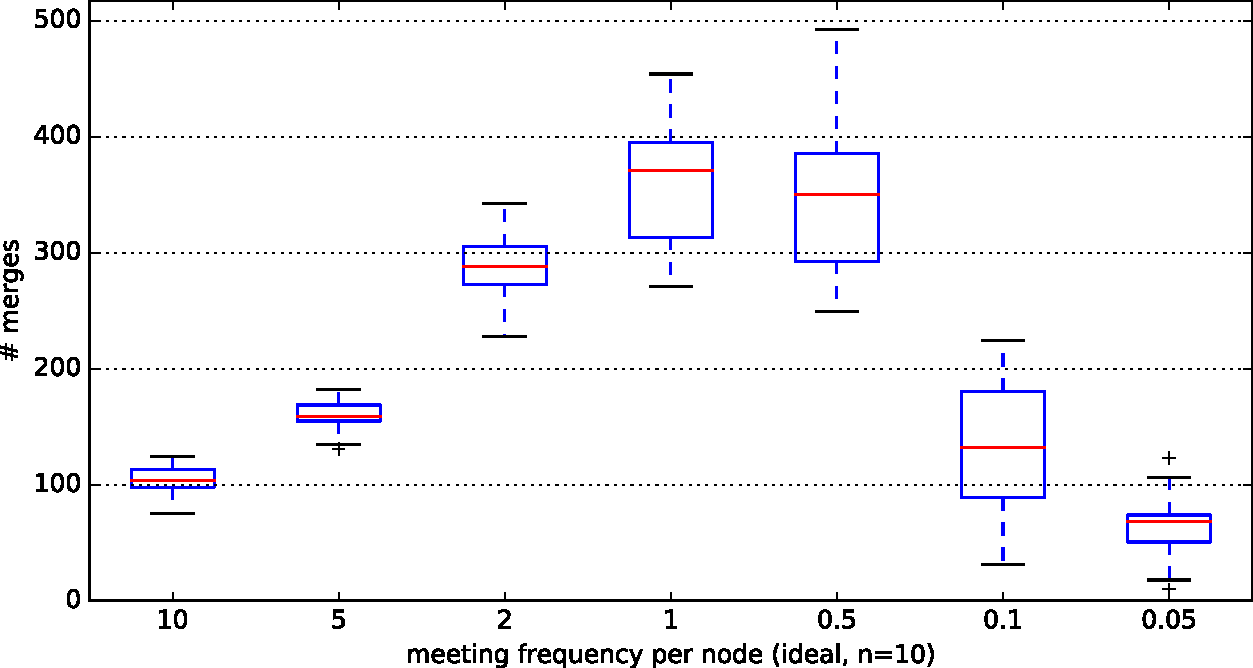
\includegraphics[width=\linewidth]{img_pdf/global_meeting_frequency_n=10.pdf}
  \caption{Total number of merges depending on meeting frequency per time unit with n=10}
  \label{fig:freq_n10}
\end{figure}

However, the higher the node count, the faster this communication needs to be, even if we hold constant the number of edits \textit{per network} and not per node. For n=30 (fig. \ref{fig:freq_n30}), the maximum is closer to 0.5 than 1. In a larger network, faster communication speed is required in order to get all members on the same page. In other words, without a centralized synchronization point, the probability of having to merge upon receiving a new commit in a distributed system approaches 1 as the number of participants grows, as the two nodes are likely to hold differing subsets of edits.
\begin{figure}
  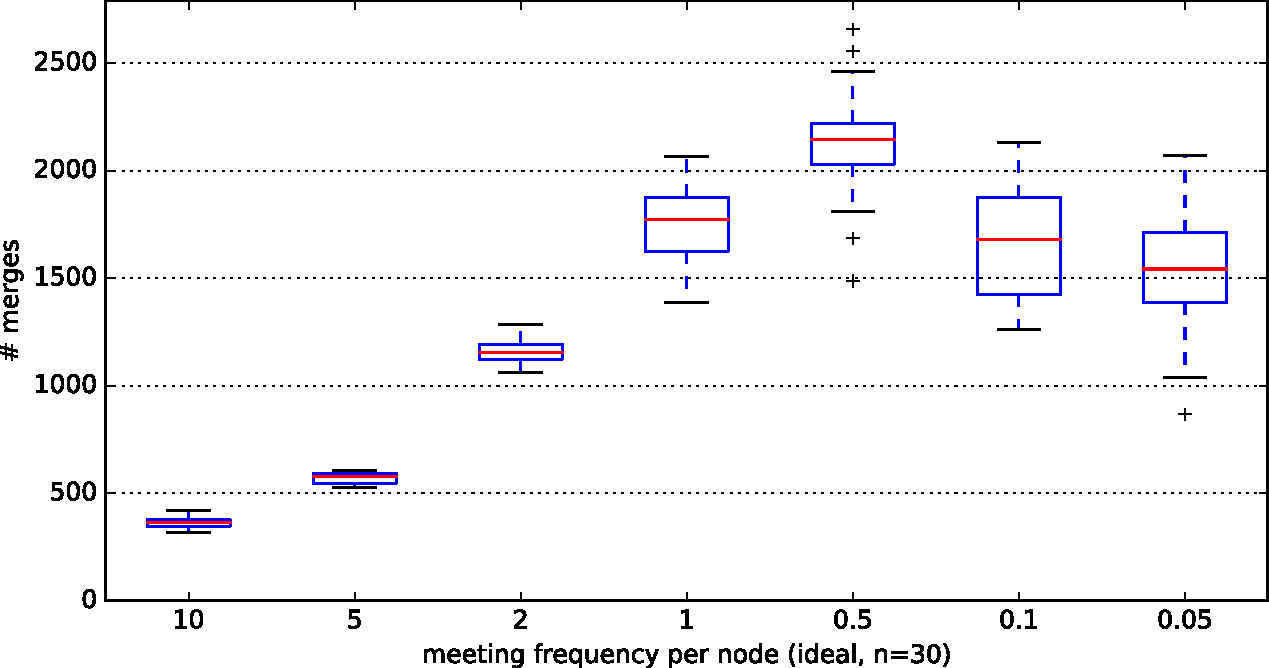
\includegraphics[width=\linewidth]{img_pdf/global_meeting_frequency_n=30.pdf}
  \caption{Total number of merges depending on meeting frequency per time unit with n=30}
  \label{fig:freq_n30}
\end{figure}

This behavior can also be seen with the default algorithm in small networks (fig. \ref{fig:freq_dumb_n10}), although with large node counts the number of merges only increases (fig. \ref{fig:freq_dumb_n30}).

\begin{figure}
  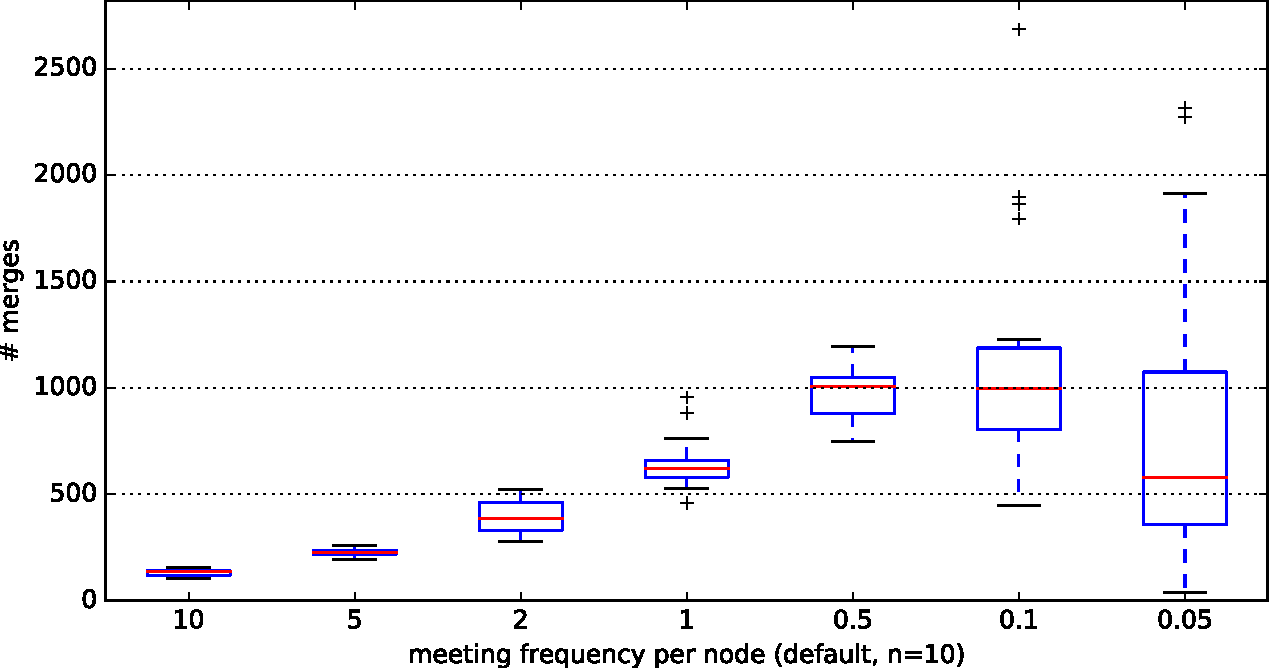
\includegraphics[width=\linewidth]{img_pdf/dumb_meeting_frequency_n=10.pdf}
  \caption{Total number of merges with the default algorithm and n=10}
  \label{fig:freq_dumb_n10}
\end{figure}
\begin{figure}
  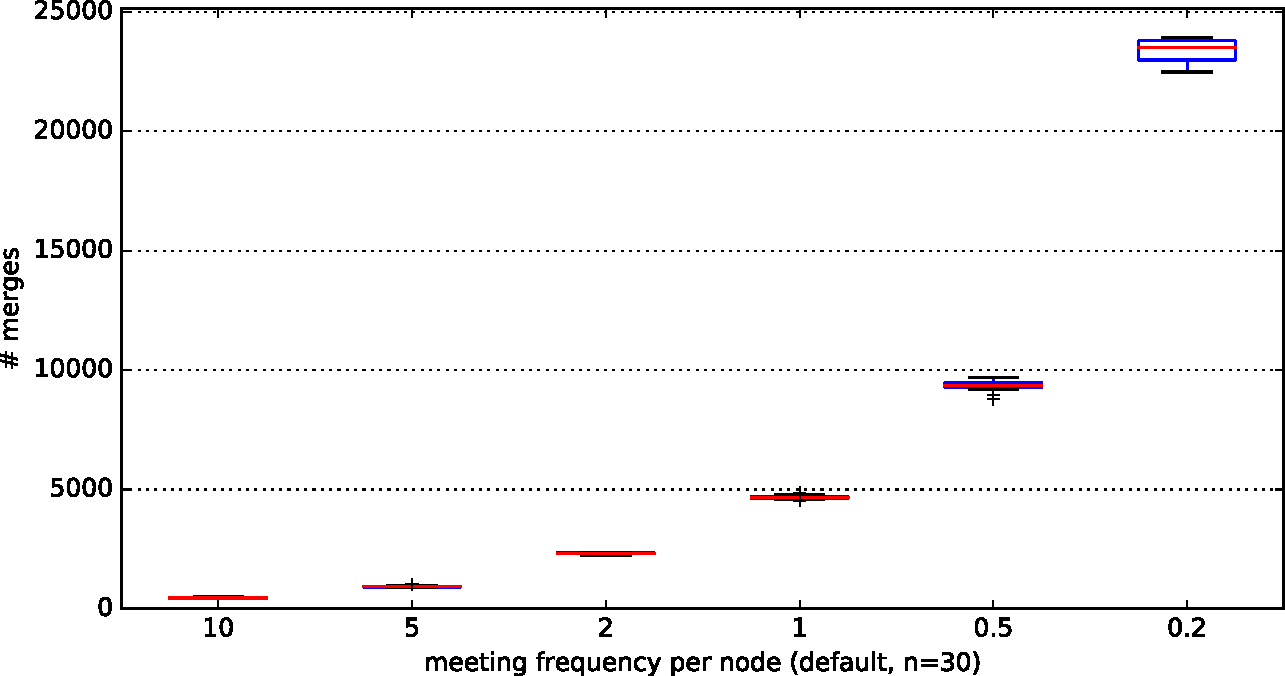
\includegraphics[width=\linewidth]{img_pdf/dumb_meeting_frequency_n=30.pdf}
  \caption{Total number of merges with the default algorithm and n=30}
  \label{fig:freq_dumb_n30}
\end{figure}

Remarkably, when keeping the total number of edits constant, the total merge count scales linearly with network size, as shown in fig. \ref{fig:n}.

\begin{figure}
  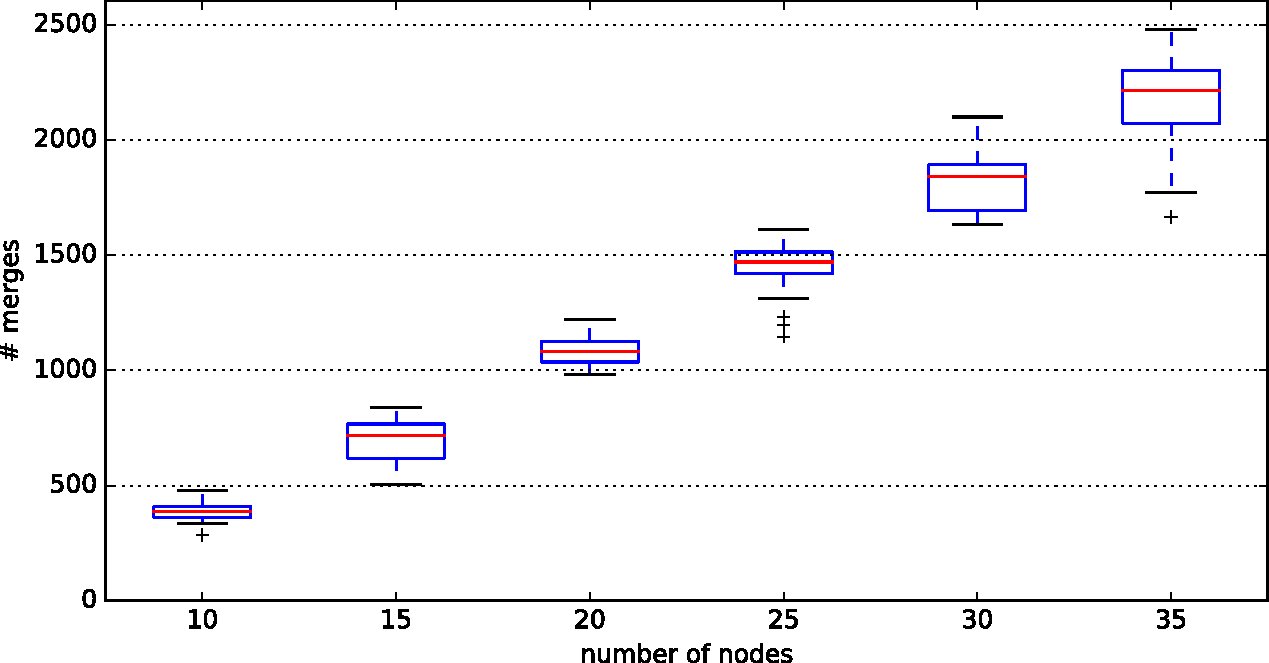
\includegraphics[width=\linewidth]{img_pdf/n_with_same_edits.pdf}
  \caption{Merge count depending on network size}
  \label{fig:n}
\end{figure}



Another interesting question concerns the communication behaviour when two nodes meet. Up until now, we assumed that at every meeting, a sender simply \textit{pushes} a packet to a receiver. Alternatively, we can assume that sender and receiver perform the \textit{merge} collaboratively (or either of them immediately distributes the result). A third model would be both nodes exchanging their current state before merging (\textit{doublepush}).

As can be seen in fig. \ref{fig:bidi_n20}, merging before parting ways is the most effective method by far. This is not surprising, as this approach is similar to the same simulation with half the node count. By making sure that every merge has to be performed by both communication partners, the doublepush scheme has the opposite effect.

% \begin{figure}
%   \includegraphics[width=\linewidth]{img_pdf/bidi_n=10.pdf}
%   \caption{Bidirectional merging with 10 nodes}
%   \label{fig:bidi_n10}
% \end{figure}
\begin{figure}
  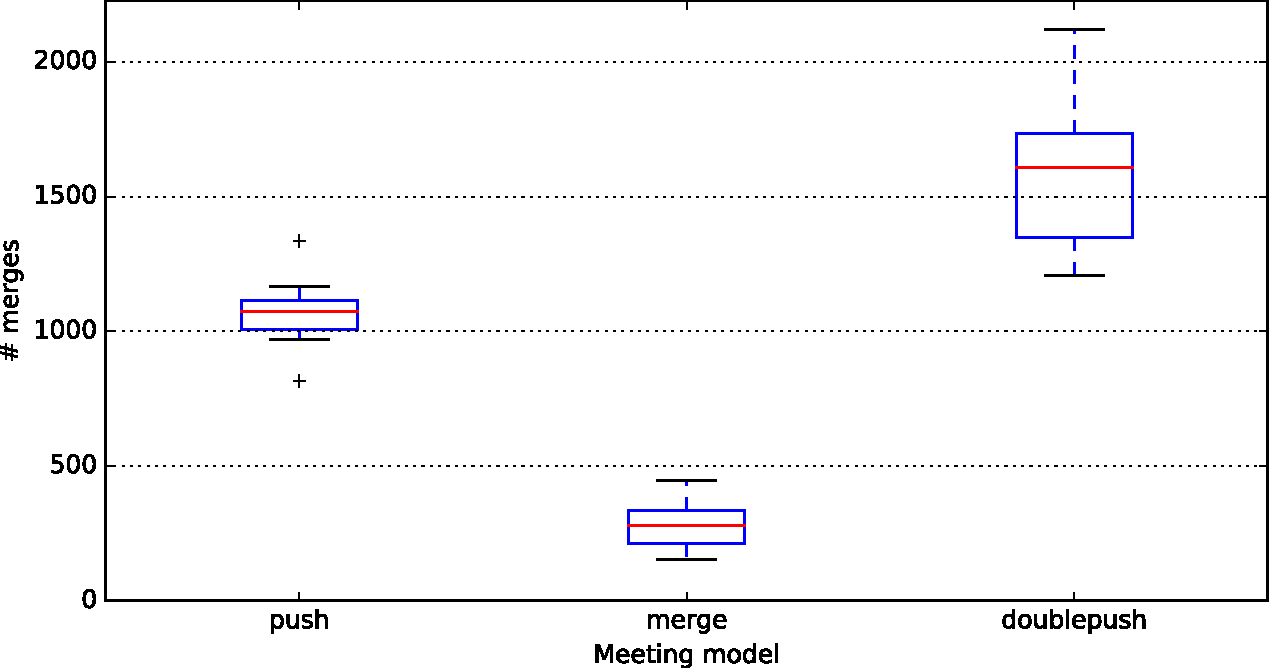
\includegraphics[width=\linewidth]{img_pdf/bidi_n=20.pdf}
  \caption{Bidirectional merging with 20 nodes}
  \label{fig:bidi_n20}
\end{figure}

\section{Consequences}

First of all, we note that the default merging algorithm currently employed in graph-based revision control system, are unsuitable even in small networks, because it is very likely that there will always be two irreconcilable newest versions, even in the absence of any new edits. This effect can be dampened by a multitude of factors, among them users stopping merging of new commits as well as users sharing the merges before parting ways.

With an ideal merging function, the number of merge actions grows linearly with network size. This is quite acceptable, considering that this means that the effort every node has to put into the system on average stays fixed even when the network grows in size.

We have also shown that the detrimental effects of using a DTN as a communication challenge vanish in extremely slow or extremely fast networks, the latter being equivalent to a low-latency server. This is the reason why the high costs are mitigated in current server-based setups.

\section{Outlook}

In this paper, we assume a very abstract view of the merging process, not delving into the actual implementation. Classification, analysis and improvement of actual merging implementations is needed in order to fulfill the abstract properties we have used in this paper, such as being very close to the \textit{ideal} merging system whenever possible.

We assume a very generic and simple movement model. While we do not expect fundamentally different results in other network forms, another movement model may allow a multiple of the network size. For instance, if a local cluster of nodes communicates in near-real time, it can likely be regarded just like one single node. The movement model used here functions as a worst-case scenario.

To our knowledge, there is no actual system tackling the challenge of a totally distributed revision control system which works in a DTN. We believe the advantages in terms of scalability, easy configuration, anti-censorship and extreme reliability are worth studying and eventually building such a system. One avenue to that effect may be the adaption of patch-based revision control systems like \textit{Darcs}\cite{roundy2005darcs} to automatic communication in DTNs.

\begin{thebibliography}{1}

% \bibitem{shavitt2012arabian}
% Shavitt, Yuval and Zilberman, Noa, \emph{Arabian nights: measuring the arab internet during the 2011 events}. In IEEE Network 26.6 (2012): 75--80.

\bibitem{outage}
Dainotti, Alberto, et al., \emph{Analysis of country-wide internet outages caused by censorship.} In Proc. of the 2011 ACM SIGCOMM conference on Internet measurement conference, 2011.

\bibitem{groenevelt}
Groenevelt, Robin, Philippe Nain, and Ger Koole, \emph{The message delay in mobile ad hoc networks.}. In Performance Evaluation 62.1 (2005): 210-228.

\bibitem{demmer2008tierstore}
M. Demmer,  B. Du, and E. Brewer, \emph{TierStore: A Distributed Filesystem for Challenged Networks in Developing Regions}. In Proc. of USENIX Conference on File and Storage Technologies (FAST), 2008.

\bibitem{ahlgren2011experiments}
B. Ahlgren, B. Ohlman, E. Axelsson, and L. Brown, \emph{Subversion over OpenNetInf and CCNx}, In Proc. of IEEE Workshop on Architectures, Services and Applications for the Next Generation Internet (WASA-NGI-IV), 2011.

\bibitem{mukherjee2005fully}
P. Mukherjee, \emph{A Fully Decentralized, Peer-to-Peer Version Control System}, Ph. D. Dissertation, Technische Universit{\"a}t Darmstadt, 2011.

\bibitem{roundy2005darcs}
D. Roundy., \emph{Darcs: Distributed Version Management in Haskell}, In Proc. of ACM SIGPLAN Workshop on Haskell, 2005.

\end{thebibliography}


\end{document}
